\section{Implemented Hardware System}\label{sec:hardware}
\subsection{Hardware Equipment and Model Identification}
Table~\ref{tab:hardware} records the hardware supported by the firmware, wiring sketches, and photographs. Exact model information is retained where documented, and ambiguous identities are marked for confirmation. The photographed load cell has a readable 5~kg label, while the ESP32 development-board variant and power-source rating are not established by readable labels.

\begin{table*}[!t]
\caption{Hardware Inventory and Evidence of Component Identity}\label{tab:hardware}
\centering\small
\begin{tabularx}{\textwidth}{@{}P{0.22\textwidth}P{0.23\textwidth}Y@{}}
\toprule
Equipment & Model / specification & Role and evidence \\
\midrule
Microcontroller development board & ESP32; PlatformIO target \code{esp32dev} & Main acquisition, actuation, Wi-Fi and task scheduling. Exact board/module variant requires confirmation. \\
Optical biosensor module & MAX30102 & Red/infrared acquisition for pulse and SpO\textsubscript{2} estimates; named in code, slides, and sensor wiring. \\
Single-lead ECG front end & AD8232 & Analog signal conditioning and lead-off outputs; named in the sensor wiring, with matching firmware pins. \\
Load-cell ADC/interface & HX711 & Reads the container-load sensor; identified by firmware and wiring. \\
Load cell and hook & 5~kg capacity label; exact part number unspecified & Upper stand assembly visible in photograph~4. Mechanical mounting converts supported load to a sensing input. \\
Saline clamp servo & SG90 in wiring; MG996R in code comments & PWM output on GPIO~5. Physical model must be confirmed because the two sources disagree. \\
Syringe and oxygen-designated servos & MG996R in wiring and code comments & PWM outputs on GPIO~18 and GPIO~16. Actual torque/travel and delivered quantities were not measured in supplied records. \\
Local alarm & Active buzzer; exact part number unspecified & GPIO~4 output, named in the actuator diagram and firmware. \\
Syringe mechanism & Syringe, handmade guide, rack and gear & Photographed mechanism; syringe capacity and travel-to-volume calibration are unspecified. \\
Fluid/oxygen-related assembly & Tubing, mask, and mounted mechanical components & Visible in photographs~2, 3, and 6; exact regulator/container ratings and output flow are unspecified. \\
Structure and power & Pole, caster base, enclosure, breadboards, wiring; external 5~V actuator rail in diagram & Provides physical integration. Battery chemistry, capacity, regulator identity, and current budget require confirmation. \\
Additional photographed hardware & Motor-driver-like board, secondary controller, ultrasonic-style modules & Visible in photographs but not operated by the supplied ESP32 source. Exact models and any separate mobility firmware are unspecified. \\
\bottomrule
\end{tabularx}
\end{table*}

The presentation additionally lists an IR drop sensor, stepper motor, lead screw, LCD, rechargeable battery, and following sensor/camera. The supplied medical firmware contains no corresponding drop-counting, stepper, LCD, or following-control routines. These items are not presented as verified functioning modules in the implementation inventory.

\subsection{Electrical Interfacing and Pin Assignment}
Table~\ref{tab:pins} gives the code/wiring pin assignment. The MAX30102 communicates through SDA and SCL; the AD8232 provides an ADC input and two digital status inputs; and the HX711 uses a clock/data interface. The three servo signals use dedicated LEDC channels, while the buzzer is switched through a GPIO output.

\begin{table}[!t]
\caption{ESP32 Pin Assignment}\label{tab:pins}
\centering\footnotesize
\begin{tabularx}{\columnwidth}{@{}YP{0.18\columnwidth}P{0.30\columnwidth}@{}}
\toprule
Signal & GPIO & Interface \\
\midrule
MAX30102 SDA / SCL & 21 / 22 & I\textsuperscript{2}C, 100~kHz \\
AD8232 OUT & 34 & ADC1, channel~6 \\
AD8232 LO+ / LO$-$ & 25 / 26 & Digital inputs \\
HX711 DT / SCK & 19 / 23 & Serial data / clock \\
Saline servo & 5 & LEDC channel~1 \\
Syringe servo & 18 & LEDC channel~2 \\
Oxygen-designated servo & 16 & LEDC channel~0 \\
Active buzzer & 4 & Digital output \\
\bottomrule
\end{tabularx}
\end{table}

The supplied sensor sketch shows a 3.3~V rail and a common ground. The actuator sketch shows an external 5~V rail with servo and ESP32 grounds joined; it does not establish the supply's available current or transient performance. The diagrams also omit detailed load-cell bridge wiring, protective components, and module-specific regulator arrangements. Module voltages, I\textsuperscript{2}C electrical behavior, and power capacity therefore require verification against the actual boards and device documentation~\cite{max30102,ad8232,i2cmanual}.

\subsection{Software Environment}
The embedded program is C, with ESP-IDF as the framework and PlatformIO as the project environment. The configuration specifies the \code{espressif32} platform, \code{esp32dev} board, DIO flash mode, and a 115200-baud serial monitor. CMake requires version~3.16 or later and registers the sources under \code{src}. The saved generated SDK configuration identifies ESP-IDF~6.1.0, but the PlatformIO platform version is not pinned, so a fresh installation is not guaranteed to reproduce that toolchain exactly.

The firmware uses ESP-IDF GPIO, LEDC, I\textsuperscript{2}C, ADC, Wi-Fi, HTTP-client, SNTP, and FreeRTOS facilities. The frontend consists of static HTML, CSS, and JavaScript pages served by Firebase Hosting. Application pages use Firebase SDK~8.10.1; the doctor interface also uses Bootstrap~5.3.0 and a Chart.js CDN dependency. The default hosting welcome page uses a different Firebase SDK version and is separate from the application login page.

A configuration inconsistency affects reproducibility: \code{platformio.ini} specifies a 4~MB upload flash size, whereas the saved SDK configuration selects 2~MB. The actual board capacity must be checked and both settings made consistent before reproducing a firmware build. There are no custom tests in the supplied test directory, and no firmware build or hardware experiment is claimed as part of this report-generation process.

\subsection{Figures of the Implemented Hardware System}
Fig.~\ref{fig:prototypephotos} labels the overall structure and two important mechanical assemblies. The upper load-cell/hook supports load sensing, the tubing and mask identify the respiratory-related assembly, and the lower enclosure contains the wiring and controller area. The syringe close-up shows a rack-and-gear construction rather than a verified lead-screw drive. Fig.~\ref{fig:electronics} identifies the base electronics and electrode connections.

\begin{figure*}[!t]
\centering
\begin{minipage}[t]{0.31\textwidth}
\centering
\begin{tikzpicture}
\node[anchor=south west,inner sep=0] (pic) at (0,0) {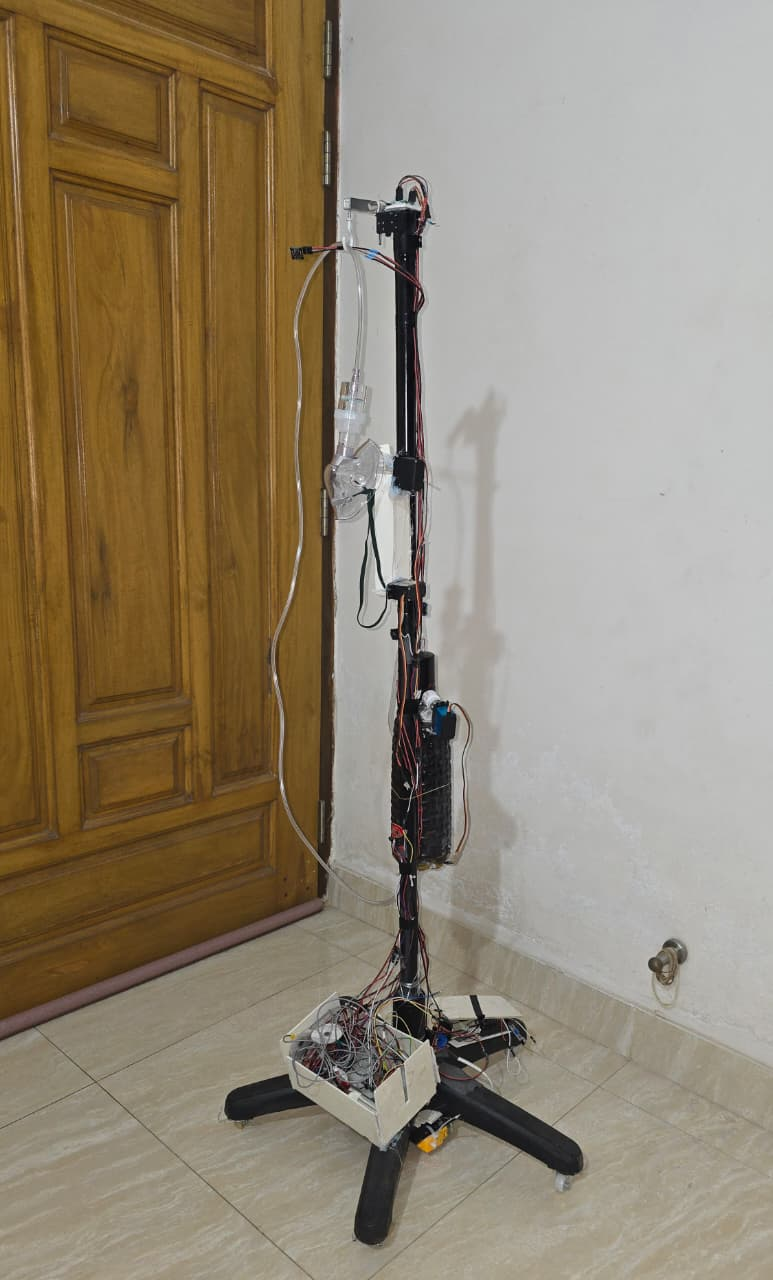
\includegraphics[width=\linewidth]{6.jpeg}};
\begin{scope}[x={(pic.south east)},y={(pic.north west)}]
\tikzset{partmarker/.style={circle,draw=black,fill=white,inner sep=2pt,font=\fontsize{8}{9}\selectfont},pointer/.style={-{Latex[length=1.5mm]},thick,preaction={draw=white,line width=2pt}}}
\node[partmarker] (a) at (0.78,0.84) {1};\draw[pointer] (a) -- (0.49,0.83);
\node[partmarker] (b) at (0.79,0.60) {2};\draw[pointer] (b) -- (0.47,0.62);
\node[partmarker] (c) at (0.79,0.38) {3};\draw[pointer] (c) -- (0.55,0.41);
\node[partmarker] (d) at (0.17,0.18) {4};\draw[pointer] (d) -- (0.46,0.17);
\node[partmarker] (e) at (0.79,0.06) {5};\draw[pointer] (e) -- (0.67,0.09);
\end{scope}
\end{tikzpicture}
\par\smallskip\footnotesize (a) Overall prototype. 1: load-cell/hook; 2: mask/tubing; 3: mounted actuation assembly; 4: electronics enclosure; 5: caster base.
\end{minipage}\hfill
\begin{minipage}[t]{0.31\textwidth}
\centering
\begin{tikzpicture}
\node[anchor=south west,inner sep=0] (pic) at (0,0) {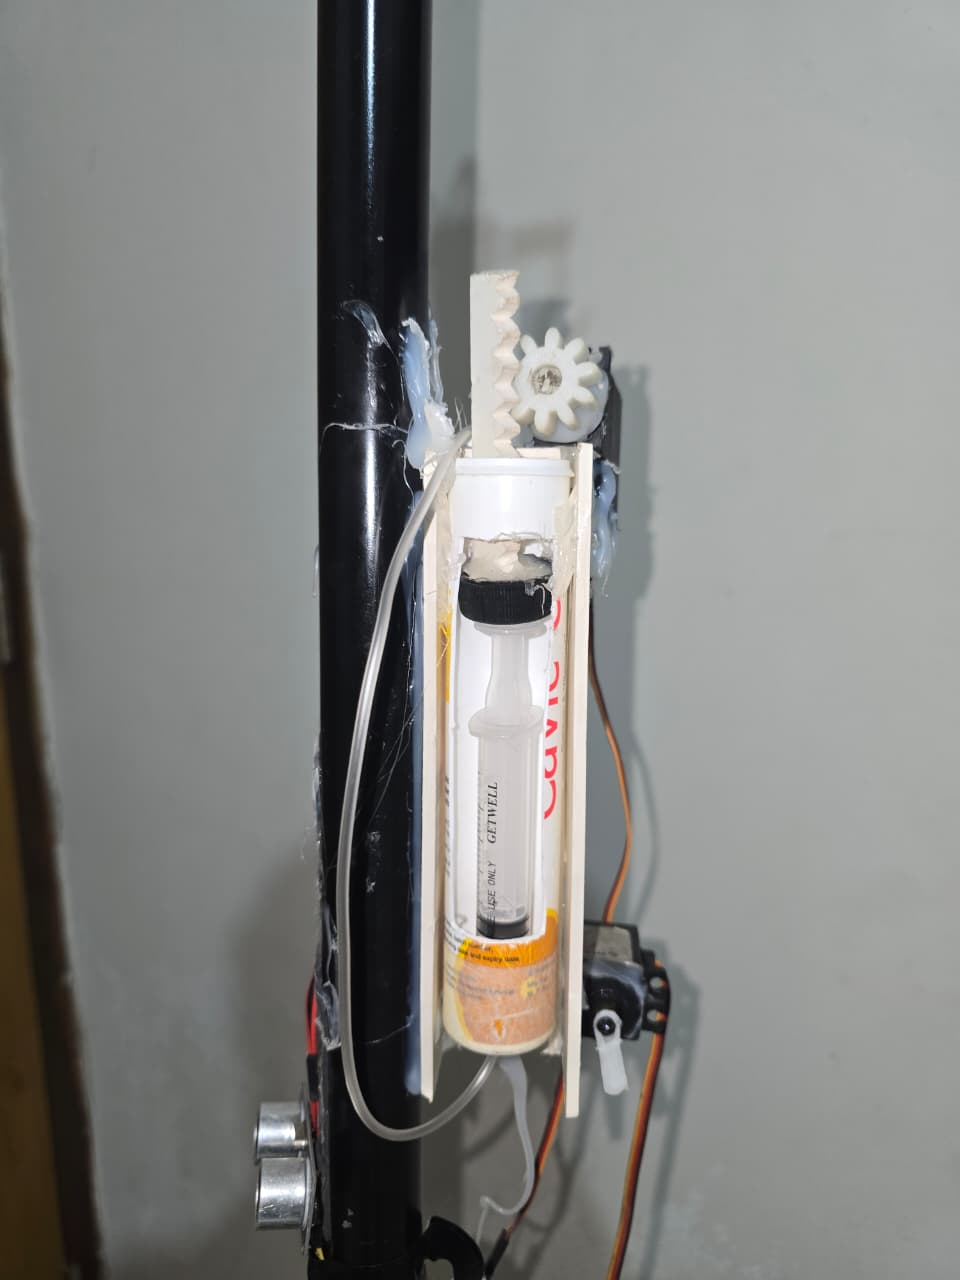
\includegraphics[width=\linewidth]{3.jpeg}};
\begin{scope}[x={(pic.south east)},y={(pic.north west)}]
\tikzset{partmarker/.style={circle,draw=black,fill=white,inner sep=2pt,font=\fontsize{8}{9}\selectfont},pointer/.style={-{Latex[length=1.5mm]},thick,preaction={draw=white,line width=2pt}}}
\node[partmarker] (a) at (0.80,0.73) {1};\draw[pointer] (a) -- (0.58,0.71);
\node[partmarker] (b) at (0.83,0.44) {2};\draw[pointer] (b) -- (0.55,0.47);
\node[partmarker] (c) at (0.88,0.19) {3};\draw[pointer] (c) -- (0.65,0.22);
\end{scope}
\end{tikzpicture}
\par\smallskip\footnotesize (b) Syringe construction. 1: rack and gear; 2: syringe/guide; 3: visible servo attachment. Photographs do not quantify delivered dose.
\end{minipage}\hfill
\begin{minipage}[t]{0.31\textwidth}
\centering
\begin{tikzpicture}
\node[anchor=south west,inner sep=0] (pic) at (0,0) {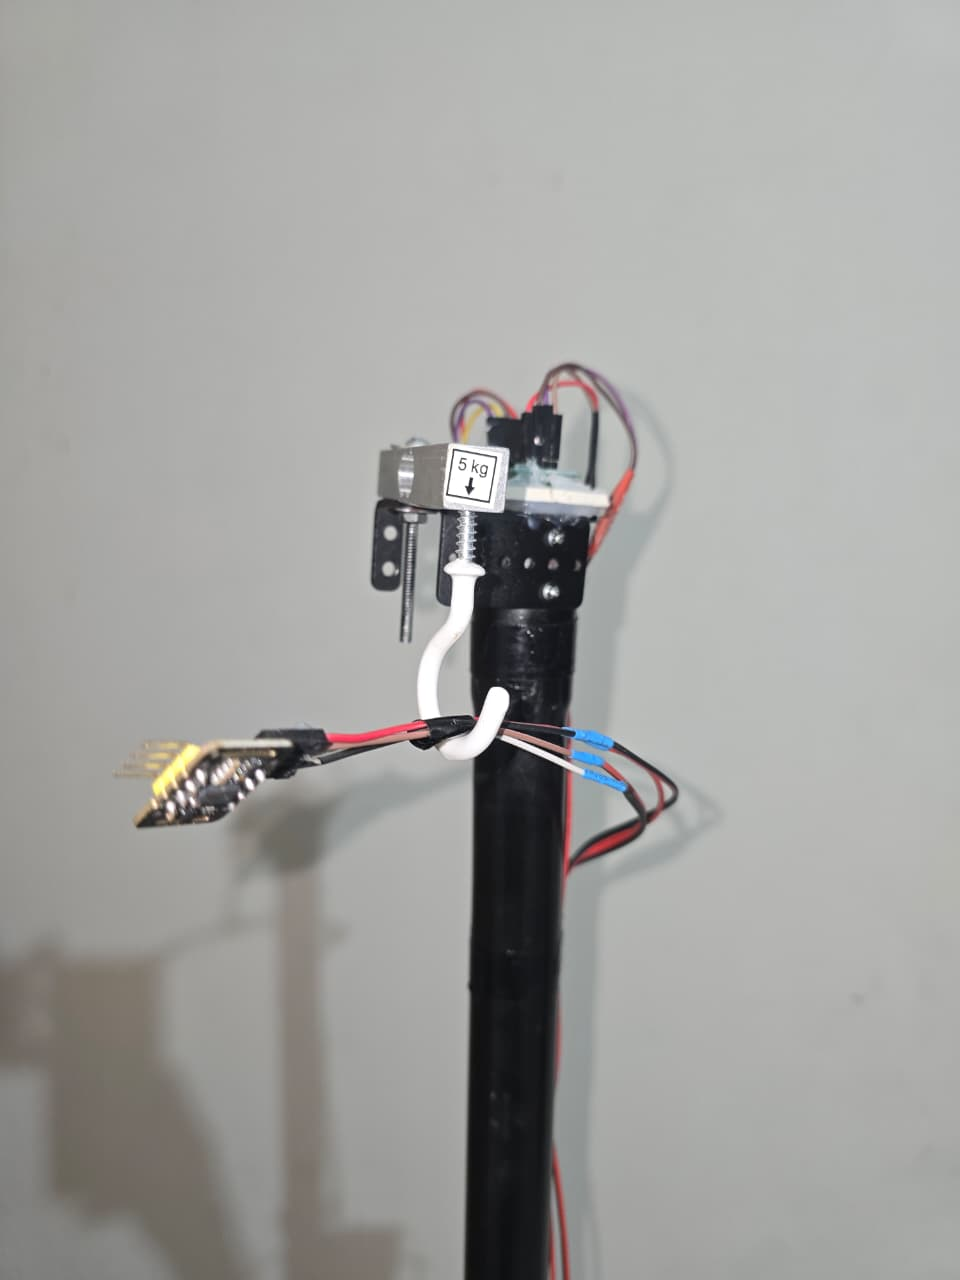
\includegraphics[width=\linewidth]{4.jpeg}};
\begin{scope}[x={(pic.south east)},y={(pic.north west)}]
\tikzset{partmarker/.style={circle,draw=black,fill=white,inner sep=2pt,font=\fontsize{8}{9}\selectfont},pointer/.style={-{Latex[length=1.5mm]},thick,preaction={draw=white,line width=2pt}}}
\node[partmarker] (a) at (0.23,0.66) {1};\draw[pointer] (a) -- (0.48,0.63);
\node[partmarker] (b) at (0.79,0.48) {2};\draw[pointer] (b) -- (0.49,0.46);
\node[partmarker] (c) at (0.82,0.75) {3};\draw[pointer] (c) -- (0.62,0.65);
\end{scope}
\end{tikzpicture}
\par\smallskip\footnotesize (c) Load sensing mount. 1: load cell labeled 5~kg; 2: hanging hook; 3: wiring and support electronics.
\end{minipage}
\caption{Annotated photographs supplied with the project: overall view (photograph~6), syringe assembly (photograph~3), and load-cell mount (photograph~4). Numbered callouts identify visible parts without assigning unreadable model labels.}\label{fig:prototypephotos}
\end{figure*}

\begin{figure}[!t]
\centering
\begin{tikzpicture}
\node[anchor=south west,inner sep=0] (pic) at (0,0) {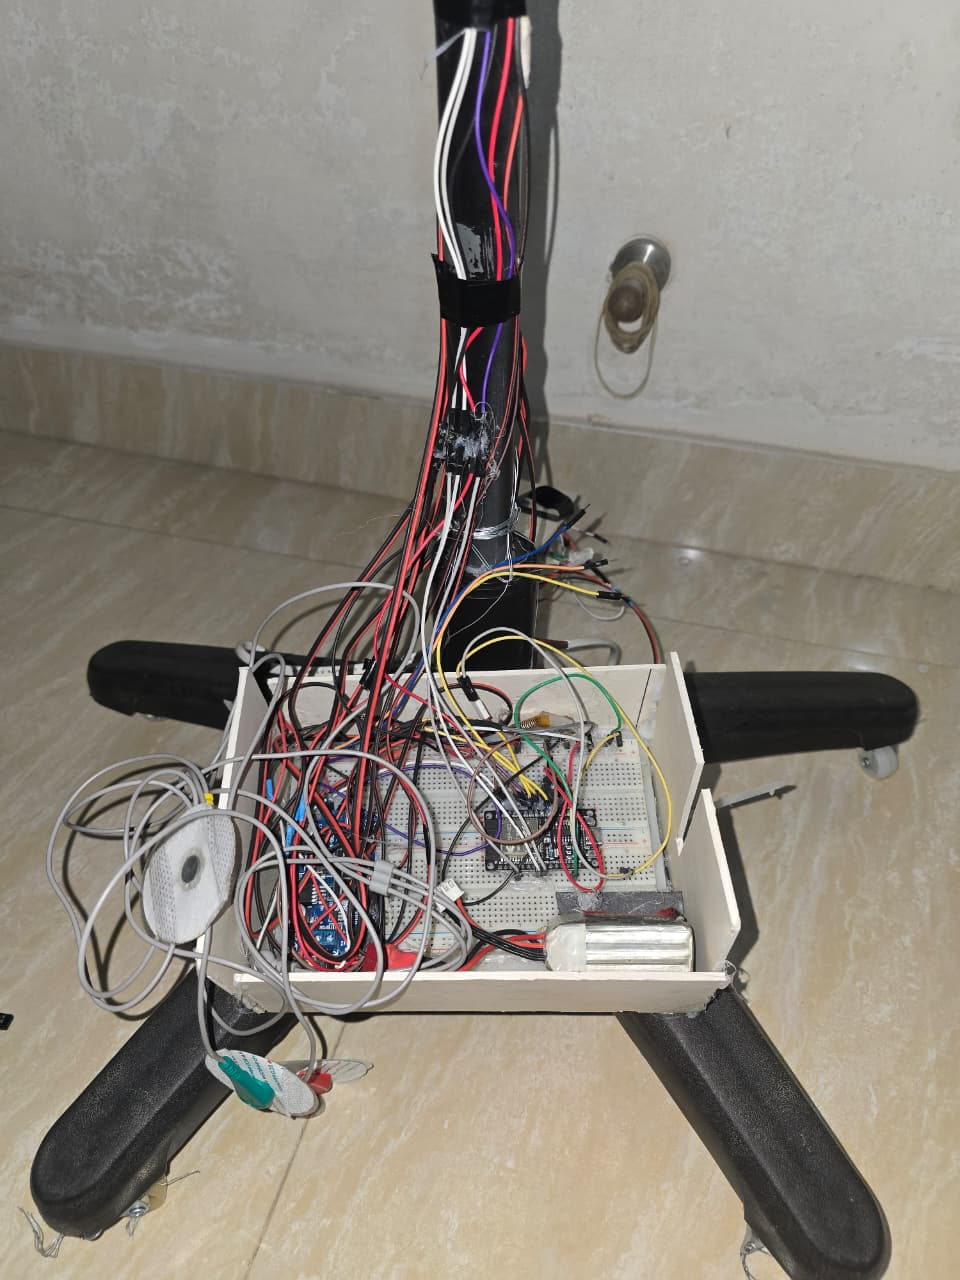
\includegraphics[width=0.83\columnwidth]{1.jpeg}};
\begin{scope}[x={(pic.south east)},y={(pic.north west)}]
\tikzset{partmarker/.style={circle,draw=black,fill=white,inner sep=2pt,font=\fontsize{8}{9}\selectfont},pointer/.style={-{Latex[length=1.5mm]},thick,preaction={draw=white,line width=2pt}}}
\node[partmarker] (a) at (0.86,0.44) {1};\draw[pointer] (a) -- (0.56,0.36);
\node[partmarker] (b) at (0.82,0.19) {2};\draw[pointer] (b) -- (0.66,0.30);
\node[partmarker] (c) at (0.13,0.16) {3};\draw[pointer] (c) -- (0.26,0.16);
\end{scope}
\end{tikzpicture}
\caption{Base electronics in photograph~1. 1: controller-board area; 2: breadboard wiring; 3: electrode pads/cables. Wiring obscures some labels, so exact component identities are taken from the source/wiring inventory rather than inferred from this view.}\label{fig:electronics}
\end{figure}


